%%%%%%%%%%%%%%%%%%%%%%%%%%%%%%%%%%%%%%%%%%%%%%%%%%%
%%% EVALUACION
%%%%%%%%%%%%%%%%%%%%%%%%%%%%%%%%%%%%%%%%%%%%%%%%%%%

\chapter{Evaluaci�n y discusi�n}
\fancyhead[RE]{\textsc{CAP�TULO} \thechapter. Evaluaci�n}
\label{ch:Evaluacion}

\todo{Explicar proceso de evaluaci�n con digramas: ShuffleSplit + Crossvalidation}
\noindent Este cap�tulo describe la metodolog�a utilizada para evaluar el sistema/m�todo o caso de estudio propuesto, a la vez que presenta los resultados obtenidos en la evaluaci�n de las diferentes tareas y sobre colecciones de evaluaci�n de distintos dominios. Algunos ejemplos de secciones pueden ser estos:

\section{Metodolog�a de evaluaci�n}
\label{sec:Met_Eval}

\subsection{M�tricas de evaluaci�n}
\label{sec:Col_Eval}

\noindent Para la evaluaci�n de los resultados en clasificaci�n textual o de documentos se utiliza com�nmente la matriz de confusi�n. Se trata de una una herramienta que representa en cada columna el n�mero de predicciones de cada clase, mientras que cada fila representa a las instancias en la clase real. En la siguiente imagen se presenta un esquema de la matriz de confusi�n:

\begin{center}
	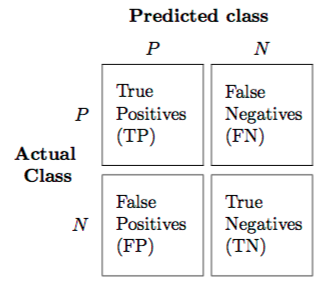
\includegraphics[width=0.5\textwidth]{imagenes/confusion_matrix_1.png} %[width=4cm,,keepaspectratio]
	\captionof{figure}{Matriz de confusi�n}	
\end{center}

Esta tabla est� formada por verdaderos positivos, verdaderos negativos, falsos positivos y falsos negativos. De este modo, si un documento es clasificado por el sistema autom�tico en la misma categor�a que la clasificaci�n manual, se considerar� como un verdadero positivo o negativo (\textit{True Positive}, TP o \textit{True Negative}, TN), mientras que si el documento es clasificado por el sistema con una categor�a diferente, se estar� ante un falso negativo o falso positivo (\textit{False Positive}, FP o \textit{False Negative}, FN).Utilizando estos cuatro componentes se calculas las medidas principales para evaluar los resultados:

\begin{itemize}
	\itemsep0em 
	\item Tasa de acierto o exactitud (\textit{accuracy}): representa el porcentaje de aciertos en relaci�n a todos los documentos clasificados.
	\[\textit{Accuracy}=\frac{TP+TN}{TP+FP+TN+FN}\]
	\item Precisi�n: representa la fracci�n de asignaciones correctas frente al total de asignaciones positivas realizadas para esa clase. Es decir, realiza una medida de la tasa de acierto para un valor de la clase.
	\[Precision=\frac{TP}{TP+FP}\]
	\item Cobertura (\textit{recall}): representa la fracci�n de asignaciones positivas respecto al conjunto real de elementos pertenecientes a la clase. Es decir, realiza una medida de la capacidad que tiene el clasificador de detectar elementos de esa clase.
	\[Cobertura=\frac{TP}{TP+FN}\]
	\item Medida-F: combina las medidas de precision y cobertura.
	\[Medida-F=\frac{2xprecisionxcobertura}{precision+cobertura}\]
\end{itemize}


\subsection{Colecci�n de evaluaci�n}
\label{sec:Col_Eval}

\subsection{L�neas base (\textit{baseline})}
\label{sec:Col_Eval}

\subsection{Experimento 1: Separaci�n 30-70 (+ optimizaci�n f1)}
\label{sec:Col_Eval}

\subsection{Experimento 2: Aplicar crossfold a todo sin tunear y con los par�metros por defecto}
\label{sec:Col_Eval}

\section{Experimento 1 (Presentaci�n de resultados y discusi�n)}
\label{sec:Metric_Eval}

\section{Experimento 2 (Presentaci�n de resultados y discusi�n)}
\label{sec:Col_Eval}

\section{Efecto del desbalanceo de la clase}
\label{sec:Resultados}



